% DO NOT COMPILE THIS FILE DIRECTLY!
% This is included by the other .tex files.

\begin{frame}[t,plain]
\titlepage
\end{frame}

\lstset{%
        language=bash,
        backgroundcolor=\color{gray!25},
        basicstyle=\ttfamily,
        breaklines=true,
        columns=fullflexible
    }


\begin{frame}
    \frametitle{Reported fraud}
    \framesubtitle{Detoured invoices}
    \begin{itemize}
        \item Supplier sends payment reminders to customers
       \item Customer answers that he paid,showing a proof of payment
        \item Supplier says that it is not his bank account details
    \end{itemize}
\end{frame}

\begin{frame}
    \frametitle{Reported fraud}
    \framesubtitle{Detoured invoices}
    \begin{block}{Open questions}
        \begin{itemize}
            \item Was the invoice created from scratch?
                \begin{itemize}
                    \item By the accounting system itself?
                    \item By a third party tool?
                \end{itemize}
            \item By a manipulation of an existing invoice
                \begin{itemize}
                    \item By the accounting system itself?
                    \item By a third party tool?
                    \begin{itemize}
                        \item Where was the original invoice created?
                        \item Where was it intercepted?
                        \item Under which form was it intercepted? (scan, office documents)
                    \end{itemize}
                \end{itemize}
        \end{itemize}
    \end{block}
\end{frame}

\begin{frame}
    \frametitle{PDF internals}
    \framesubtitle{PDF data structure}
    \begin{columns}
        \begin{column}{0.15\textwidth}
                \begin{tabular}{|l|}
                    \hline
                    \%PDF-1.5\\
                     \hline
                    1 0 obj\\
                ...\\
                endobj\\
                \hline
                2 0 obj\\
                ...\\
                endobj\\
                \hline
                ... ... obj\\
                ...\\
                endobj\\
            \end{tabular}
        \end{column}
        \begin{column}{0.5\textwidth}
            \begin{tabular}{|l|}
                obj  ... ... \\
                /Type /XRef\\
                /Index [0 113]\\
                /Size 113\\
                /W [1 3 1]\\
                /Root 110 0 R\\
                %/Info 111 0 R \\
                /ID [$<$C173A17AE5$>$ ...]\\
                \hline
                startxref offset\\
                \hline
                \%\%EOF\\
                \hline
            \end{tabular}
        \end{column}
    \end{columns}
\end{frame}

\begin{frame}
    \frametitle{PDF internals}
    \framesubtitle{Why bothering with these details?}
    because of ...
    \begin{itemize}
        \item Many different PDF format variants
        \item \url{www.adobe.com/devnet/pdf/pdf_reference_archive.html}
        \item Not all tools interpret them correctly
        \item Tools strip potential valuable information
        \begin{itemize}
            \item Comments left by the creator software
            \item Generation IDs $\to$ track original files
            \item Manipulation left overs of the "attacker"
        \end{itemize}
    \end{itemize}
\end{frame}

\begin{frame}
    \frametitle{Detoured invoices}
    \framesubtitle{Practical invoice.pdf analysis}
    \begin{block}{Data to be analyzed}
        \begin{tabular}{ll}
            Filename &   invoice.pdf\\
            Number of bytes & 27758\\
            MD5 hash &  04a18e4a2b3baf08bd5cb33121842b22
        \end{tabular}
    \end{block}
    \begin{block}{Questions}
        \begin{itemize}
            \item What version has the PDF?
            \item How many objects the PDF has?
            \item What value has is the startxref offset?
            \item What is at is location?
            \item How many objects are in the xref table?
        \end{itemize}
    \end{block}
\end{frame}


\begin{frame}[fragile]
    \frametitle{Detoured invoices}
    \framesubtitle{Practical invoice.pdf analysis}
    \begin{block}{Data to be analyzed}
        \begin{tabular}{ll}
            Filename &   invoice.pdf\\
            Number of bytes & 27758\\
            MD5 hash &  04a18e4a2b3baf08bd5cb33121842b22
        \end{tabular}
    \end{block}

    \begin{block}{Getting PDF version with standard unix tools}
    \begin{lstlisting}
file invoice.pdf

head -c 9 invoice.pdf
    \end{lstlisting}
    \end{block}
    \begin{block}{Using pdfid.py from Didier Stevens}
        \begin{lstlisting}
pdfid.py invoice.pdf
        \end{lstlisting}
    \end{block}
\end{frame}


\begin{frame}[fragile]
    \frametitle{Detoured invoices}
    \framesubtitle{Practical invoice.pdf analysis}
    \begin{block}{Data to be analyzed}
        \begin{tabular}{ll}
            Filename &   invoice.pdf\\
            Number of bytes & 27758\\
            MD5 hash &  04a18e4a2b3baf08bd5cb33121842b22
        \end{tabular}
    \end{block}

    \begin{block}{Counting objects with standard unix tools}
    \begin{lstlisting}
strings invoice.pdf  | grep "endobj" | wc -l
    \end{lstlisting}
    \end{block}
    \begin{block}{Using pdfid.py from Didier Stevens}
        \begin{lstlisting}
pdfid.py invoice.pdf
        \end{lstlisting}
    \end{block}
\end{frame}

\begin{frame}[fragile]
    \frametitle{Detoured invoices}
    \framesubtitle{Practical invoice.pdf analysis}
    \begin{block}{Data to be analyzed}
        \begin{tabular}{ll}
            Filename &   invoice.pdf\\
            Number of bytes & 27758\\
            MD5 hash &  04a18e4a2b3baf08bd5cb33121842b22
        \end{tabular}
    \end{block}

    \begin{block}{Getting the startxref offset with standard unix tools}
        \begin{lstlisting}
OFFSET=`strings invoice.pdf | grep -A 1  "startxref"  | tail -n 1`
        \end{lstlisting}
    \end{block}
\end{frame}

\begin{frame}[fragile]
    \frametitle{Detoured invoices}
    \framesubtitle{Practical invoice.pdf analysis}
    \begin{block}{Data to be analyzed}
        \begin{tabular}{ll}
            Filename &   invoice.pdf\\
            Number of bytes & 27758\\
            MD5 hash &  04a18e4a2b3baf08bd5cb33121842b22
        \end{tabular}
    \end{block}

    \begin{block}{Determining xref table with standard unix tools}
        \begin{lstlisting}
        OFFSET=`strings invoice.pdf | grep -A 1  "startxref"  | tail -n 1`
        dd if=invoice.pdf bs=1 skip=$OFFSET | less
        \end{lstlisting}
    \end{block}
\end{frame}


\begin{frame}[fragile]
    \frametitle{Detoured invoices}
    \framesubtitle{Practical invoice.pdf analysis}
    \begin{block}{Data to be analyzed}
        \begin{tabular}{ll}
            Filename &   invoice.pdf\\
            Number of bytes & 27758\\
            MD5 hash &  04a18e4a2b3baf08bd5cb33121842b22
        \end{tabular}
    \end{block}

    \begin{block}{Determining the number of items in the xref table with standard unix tools}
        \begin{lstlisting}
        OFFSET=`strings invoice.pdf | grep -A 1  "startxref"  | tail -n 1`
    dd if=invoice.pdf bs=1 skip=$OFFSET | head -n 2 | tail -n 1 | cut -d ' ' -f2
    \end{lstlisting}
\end{block}
\end{frame}



\begin{frame}[fragile]
    \frametitle{Detoured invoices}
    \framesubtitle{Extracting PDF metadata with pdfinfo}
\small
    \begin{lstlisting}
pdfinfo invoice.pdf

Title:          SSMILE_prin19041715230
Creator:        SMILE_printer
Producer:       KONICA MINOLTA bizhub C458
CreationDate:   Wed Apr 17 16:23:17 2019 CEST
ModDate:        Wed Apr 17 16:23:17 2019 CEST
Page size:      595 x 841 pts
File size:      27758 bytes
PDF version:    1.4
...
    \end{lstlisting}
\end{frame}

\begin{frame}[fragile]
    \frametitle{Detoured invoices}
    \framesubtitle{Extracting PDF metadata with pdfinfo}
    \begin{block}{Open questions}
        \begin{itemize}
            \item Is the creator known?
            \item Is the producer known?
            \item Are the timestamps in a valid time frame?
            \item Does the file size correspond?
        \end{itemize}
    \end{block}

    \begin{block}{Caution}
        \begin{itemize}
            \item All elements in a PDF could be manipulated
            \item The integrity is not guaranteed
        \end{itemize}
    \end{block}
\end{frame}

\begin{frame}[fragile]
    \frametitle{PDF dissection}
    \framesubtitle{Getting an overview with the tool pdfid.py}
    \small
    \begin{lstlisting}
pdfid.py invoice.pdf

PDFiD 0.2.1 invoice.pdf
 PDF Header: %PDF-1.4
 obj                   37
 endobj                37
 stream                16
 endstream             16
 xref                   1
 trailer                1
 startxref              1
 /Page                  1
 /JavaScript            0
 /OpenAction            1
 /AcroForm              0
\end{lstlisting}
\end{frame}

\begin{frame}
    \frametitle{Checking active components}
    \begin{block}{Items frequently used to load malware}
        \begin{itemize}
            \item OpenAction
            \item JavaScript
            \item AcroForm
        \end{itemize}
    \end{block}
\end{frame}

\begin{frame}[fragile]
\frametitle{Checking active components}
\framesubtitle{OpenAction}
\begin{lstlisting}
python pdf-parser.py  -s openaction invoice.pdf
obj 37 0
 Type: /Catalog
 Referencing: 2 0 R, 34 0 R, 1 0 R

  <<
    /Type /Catalog
    /Pages 2 0 R
    /Metadata 34 0 R
    /OpenAction [ 1 0 R /Fit ]
  >>
\end{lstlisting}
\end{frame}

\begin{frame}[fragile]
    \frametitle{Checking active components}
    \framesubtitle{OpenAction}
    \begin{lstlisting}
     /OpenAction [ 1 0 R /Fit ]
    \end{lstlisting}

    \begin{tabular}{ll}
        Object number & 1\\
        Generation number & 0\\
        Indirect reference & R\\
        Fit & Display instructions\\
    \end{tabular}
\end{frame}

\begin{frame}[fragile]
\frametitle{Checking active components}
\framesubtitle{OpenAction}
What is at object 1?
\small
\begin{lstlisting}
python pdf-parser.py invoice.pdf  -o 1
obj 1 0
 Type: /Page
 Referencing: 2 0 R, 3 0 R, 4 0 R
  <<
    /Type /Page
    /Parent 2 0 R
    /MediaBox [ 0 0 595.000 841.000 ]
    /Resources
      <<
        /ProcSet [ /PDF /Text /ImageB /ImageC /ImageI ]
        ...
\end{lstlisting}
\end{frame}

\begin{frame}
    \frametitle{Detoured invoices}
    \framesubtitle{Checking document modifications}

    \begin{itemize}
        \item Tools for manipulating PDF documents: LibreOffice, Preview  on MacOS, Adobe Acrobat
        \item Low skills are needed for doing these manipulations
    \end{itemize}
    \begin{center}
        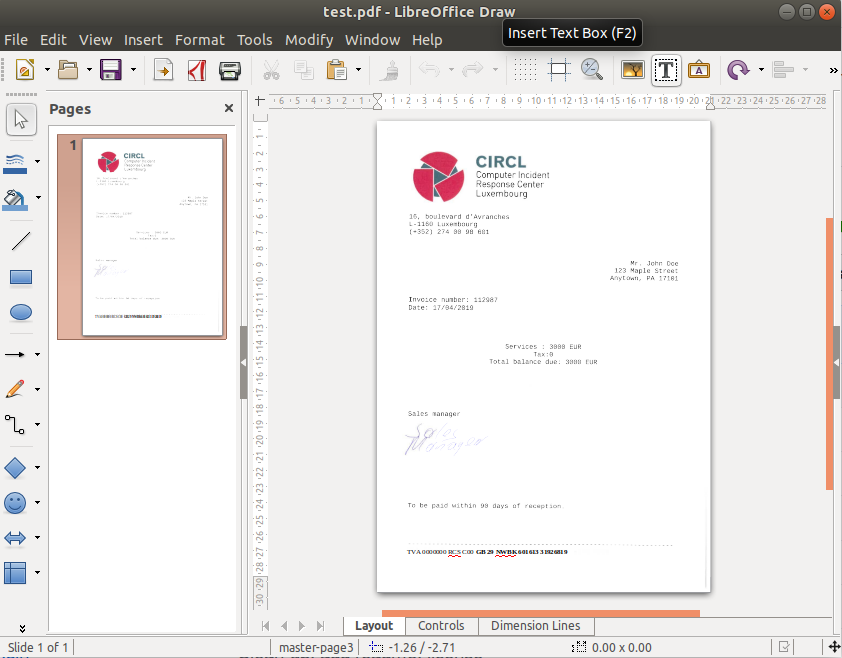
\includegraphics[scale=0.2]{libreoffice.png}
    \end{center}
\end{frame}


\begin{frame}
    \frametitle{Detoured invoices}
    \framesubtitle{Checking document modifications}

    \begin{itemize}
	\item Insert text boxes (add new bank account details, delivery addresses, ...)
	\item Adding overlays in the picture $\to$ hide some parts
	\item Add some signature scans
	\item ...
    \end{itemize}
\end{frame}

\begin{frame}
    \frametitle{Detoured invoices}
    \framesubtitle{Checking document modifications}
    \begin{center}
        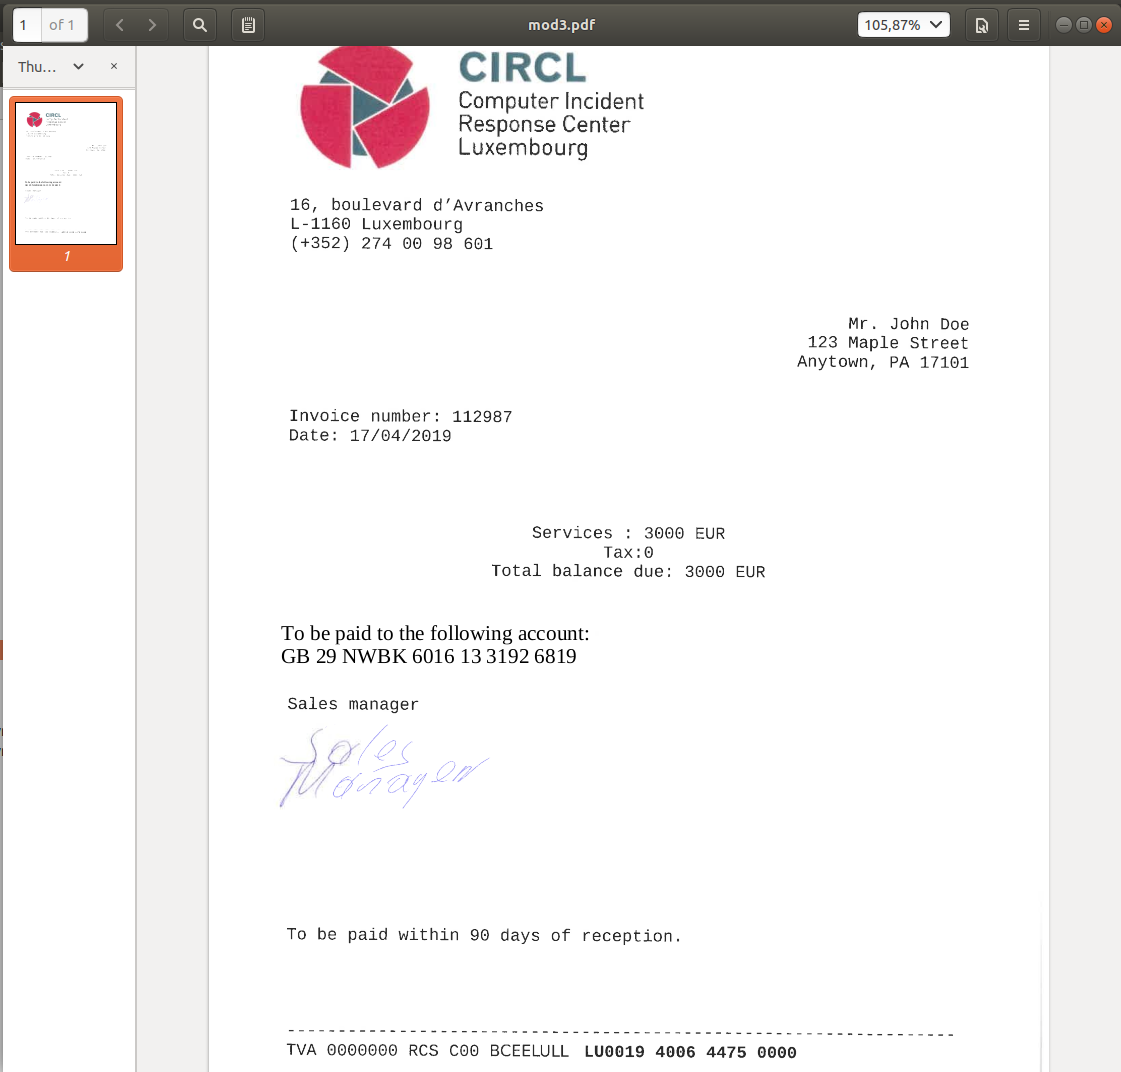
\includegraphics[scale=0.15]{add.png}
    \end{center}
\end{frame}

\begin{frame}[fragile]
    \frametitle{Detoured invoices}
    \framesubtitle{Checking document modifications}

    Checking for added text boxes
    \begin{lstlisting}
pdf-parser.py  -s /fontfile mod1.pdf

    obj 56 0
 Type: /FontDescriptor
 Referencing: 54 0 R
  <<
    /Type /FontDescriptor
    /FontName /CAAAAA+LiberationSerif-Bold
    /Flags 4
    /FontFile2 54 0 R
  >>
    \end{lstlisting}
\end{frame}


\begin{frame}[fragile]
    \frametitle{Detoured invoices}
    \framesubtitle{Checking document modifications}
    \begin{itemize}
        \item Which font descriptor corresponds to what?
        \item Dump the font file
        \item Display the glyphs
        \item Check the coordinates
        \item or ...
        \item Deactivate it and visualize
    \end{itemize}
\end{frame}

\begin{frame}[fragile]
    \frametitle{Detoured invoices}
    \framesubtitle{Checking document modifications}
    \begin{lstlisting}
        cat mod1.pdf | sed 's/58 0 obj/99 0 obj/g'  > out.pdf
    \end{lstlisting}
    \begin{center}
        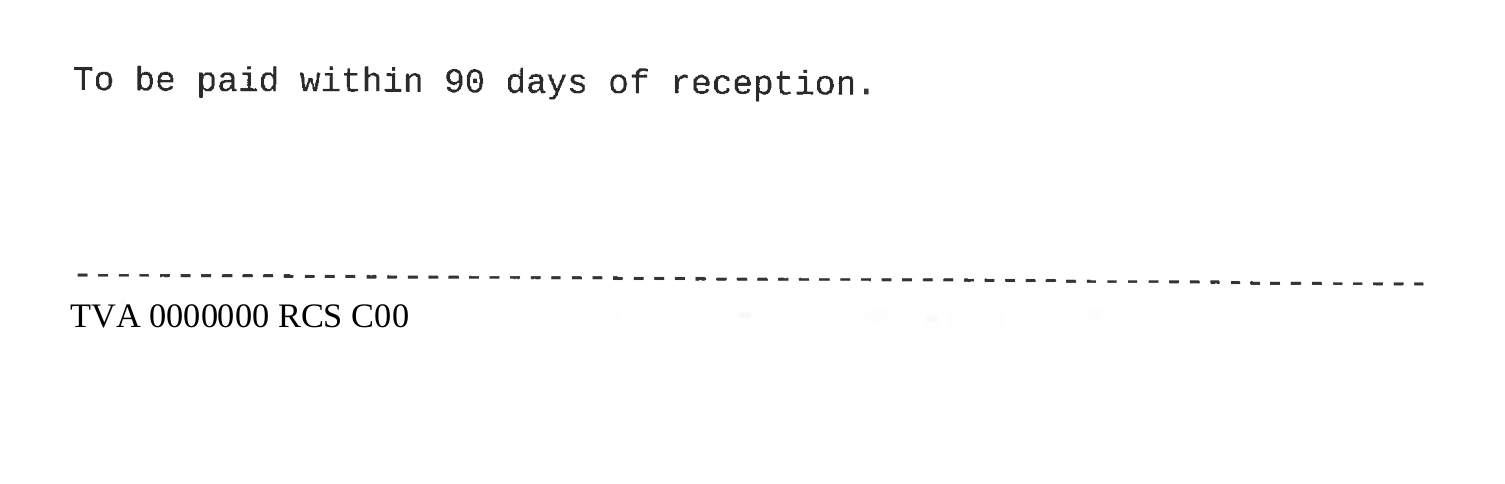
\includegraphics[scale=0.20]{account.png}
    \end{center}
\end{frame}

\begin{frame}
    \frametitle{Detoured invoices}
    \framesubtitle{Adding signature scans}
    \begin{center}
        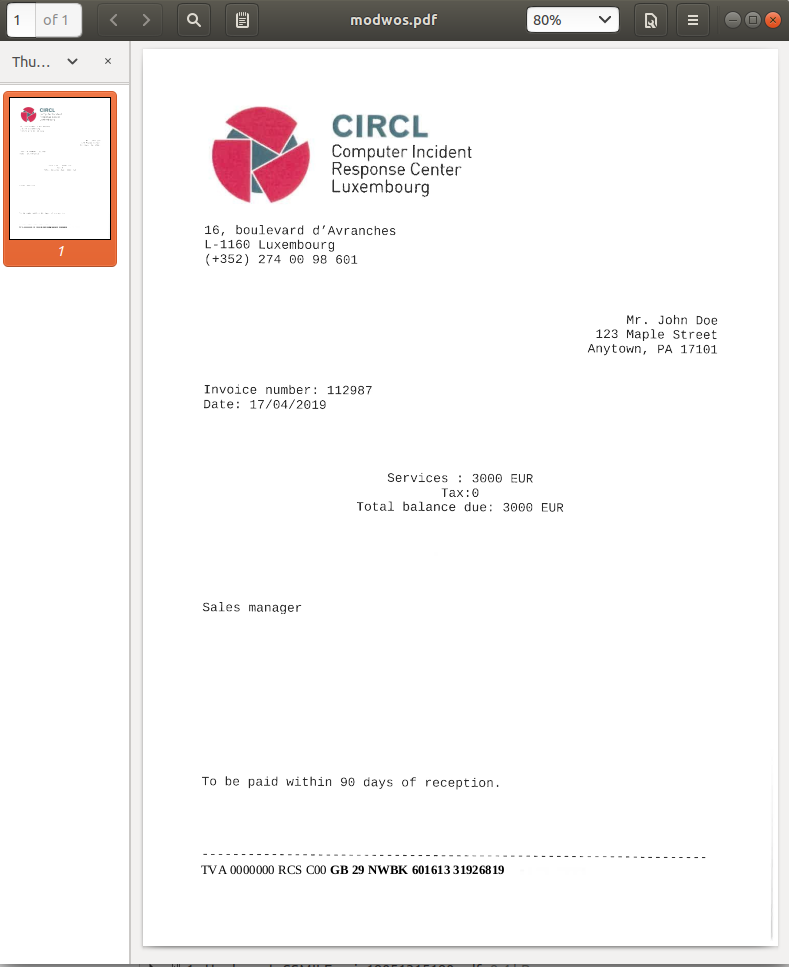
\includegraphics[scale=0.15]{wos.png}
    \end{center}
\end{frame}

\begin{frame}[fragile]
    \frametitle{Detoured invoices}
    \framesubtitle{Adding signature scans}
    \begin{center}
        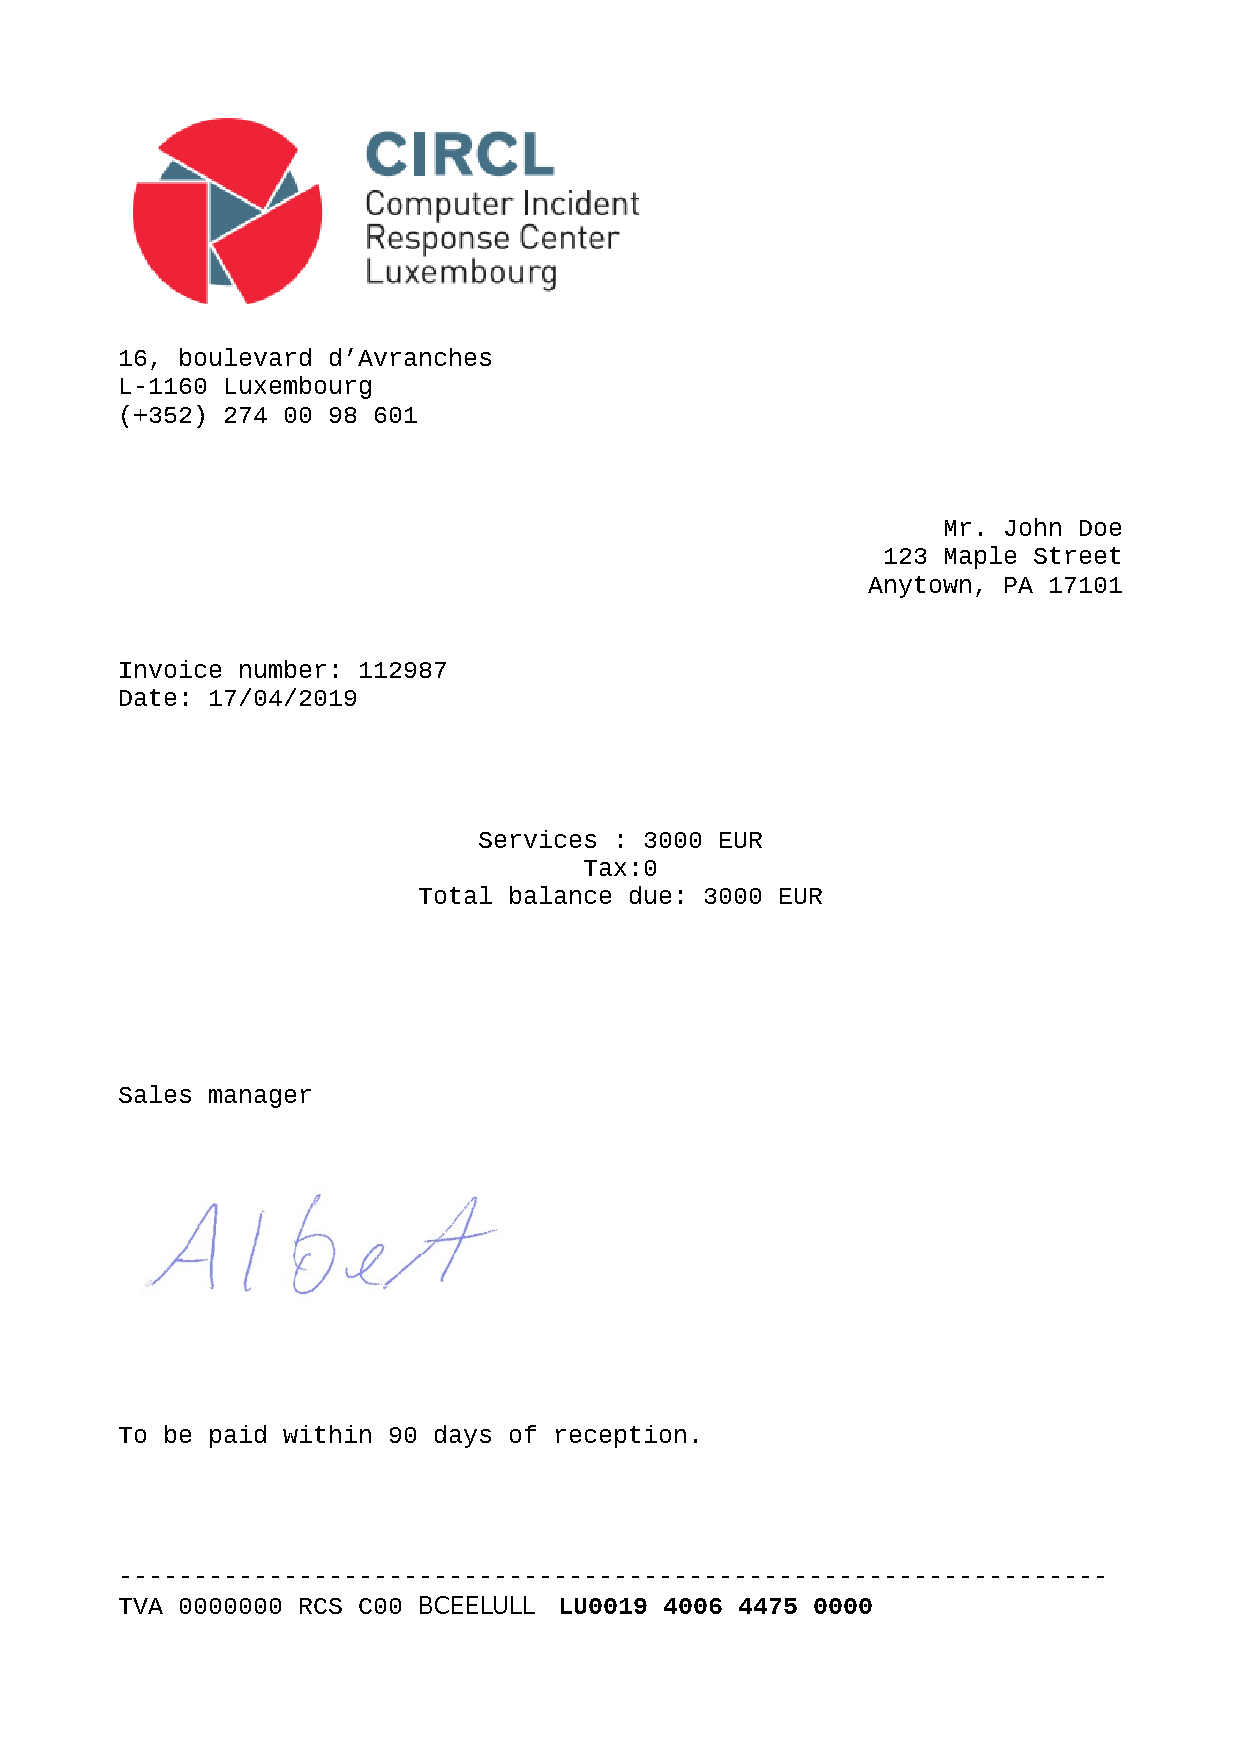
\includegraphics[scale=0.15]{samples/invoice2.pdf}
    \end{center}
\end{frame}


\begin{frame}[fragile]
    \frametitle{Detoured invoices}
    \framesubtitle{Adding signature scans}
    Search for included images
    \begin{lstlisting}
pdf-parser.py  -s /image invoice2.pdf

obj 5 0
 Type: /XObject
 Referencing: 7 0 R
 Contains stream

  <<
    /Type /XObject
    /Subtype /Image
    /Width 433
    /Height 180
    \end{lstlisting}
\end{frame}


\begin{frame}[fragile]
    \frametitle{Detoured invoices}
    \framesubtitle{Adding signature scans}

Extract the image from the pdf document

\begin{lstlisting}
pdf-parser.py -o 5 invoice2.pdf -d signature.png
\end{lstlisting}

Check the image

\begin{lstlisting}
display signature.png
\end{lstlisting}


\end{frame}

\begin{frame}
    \frametitle{Detoured invoices}
    \frametitle{What can be shared?}
    \begin{itemize}
        \item  File meta information
            \begin{itemize}
                \item Did other recipients received it?
                \item Is it in a backups?
                \item Was it in mailboxes?
                \item Is it in shadow copies
                \item ...
            \end{itemize}
        \item Timestamps $\to$ get a time range of operations
        \item Bank account details
        \begin{itemize}
            \item Prevent other transfers
            \item Correlate cases
        \end{itemize}
    \end{itemize}
\end{frame}
\small
%TODO office365
%Observed cases. Change of bank accounts, change of delivery addresses
%Ranom ideas
%Elevator industry case -> tracking the attacker with yara rules
%Leaked documents 
